\documentclass{article}
\usepackage{polski}
\usepackage{float}
\usepackage{amsmath, amssymb}
\usepackage{graphicx}
\usepackage{geometry}
\graphicspath{ {./plots/} }

\title{Sprawozdanie 3 - Algorytmy Optymalizacji Dyskretnej}
\author{Michał Kallas}
\date{16 grudnia 2024}

\begin{document}

\maketitle

\section{Wstęp}
Celem zadania było zaimplementowanie i porównanie różnych wariantów algorytmu Dijkstry do wyznaczania najkrótszych ścieżek w grafach skierowanych z nieujemnymi wagami łuków.
Porównanie obejmuje trzy wersje algorytmu:
\begin{itemize}
    \item Podstawowy algorytm Dijkstry z użyciem wydajnej kolejki priorytetowej
    \item Algorytm Diala wykorzystujący $C+1$ kubełków
    \item Algorytm korzystający ze struktury Radix Heap
\end{itemize}

\section{Algorytm Dijkstry}

\subsection{Opis algorytmu}
Tak jak zostało wspomniane we wstępie, algorytm Dijkstry służy do znajdowania najkrótszych ścieżek z jednego źródłowego wierzchołka do wszystkich innych wierzchołków w grafie z nieujemnymi wagami krawędzi.
Może zapisywać poprzedników dla każdego z wierzchołków w celu odtworzenia najkrótszej ścieżki.
W tablicy dystansów zapisuje najkrótsze dystanse do danych wierzchołków. \\

\noindent Kolejne kroki algorytmu są następujące:

\begin{itemize}
    \item Inicjalizacja: ustaw odległość od źródła \( s \) do każdego wierzchołka na \( \infty \), a od \( s \) do samego siebie na 0. Dodaj wierzchołek startowy do kolejki.
    \item W każdej iteracji wybierz wierzchołek \( u \) o najmniejszej odległości, odwiedź go i zaktualizuj odległości do jego sąsiadów, jeśli ścieżka przez \( u \) jest krótsza.
    \item Powtarzaj do przetworzenia wszystkich wierzchołków.
\end{itemize}

\subsection{Analiza złożoności}
Złożoność algorytmu Dijkstry zależy od struktury danych użytej do przechowywania kolejki priorytetowej:

\begin{itemize}
    \item \textbf{Prosta struktura (np. tablica)} Złożoność czasowa wynosi $O(|V|^2 + |E|)$, jako że wybór wierzchołka ma koszt $O(|V|^2)$, a aktualizacja dystansów $O(|E|)$
    \item \textbf{Kopiec binarny} Złożoność czasowa wynosi $O((|V| + |E|) \log |V|)$, jako że operacje dodawania i usuwania wierzchołkow z kolejki mają złożoność logarytmiczną
    \item \textbf{Kopiec Fibonacciego} Złożoność czasowa wynosi $O(|V| \log |V| + |E|)$, jednak kopiec Fibonacciego to skomplikowana struktura, która wymaga złożonej, kosztownej implementacji
\end{itemize}

\section{Algorytm Diala}

\subsection{Opis algorytmu}
Algorytm Diala, to zmodyfikowana wersja algorytmu Dijkstry.
Zamiast kolejki piorytetowej, korzysta z kubełków do przechowywania wierzchołków o różnych odległościach.
W każdym takim kubełku znajdują się wierzchołki z taką samą odległością do wierzchołka startowego.
Liczba kubełków wynosi \( C + 1 \), gdzie \( C \) to maksymalny koszt krawędzi.\\

\noindent Kolejne kroki algorytmu są następujące:

\begin{itemize}
    \item Inicjalizacja: ustaw odległość od źródła \( s \) do każdego wierzchołka na \( \infty \), a od \( s \) do samego siebie na 0, przygotuj \( C+1 \) kubełków i wrzuć wierzchołek startowy do kubełka 0.
    \item Wybierz pierwszy wierzchołek z aktualnego kubełka.
    \item Jeśli jego odległość jest mniejsza niż bieżąca wartość kubełka, pomiń go.
    \item Oblicz odległości do sąsiadów wierzchołka. Jeśli są krótsze, zaktualizuj je oraz umieść sąsiadów w odpowiednich kubełkach.
    \item Przejdź do następnego kubełka, jeśli bieżący jest pusty, i powtarzaj, aż wszystkie wierzchołki zostaną przetworzone(cyklicznie).
\end{itemize}

\subsection{Analiza złożoności}
Dzięki kubełkom, jesteśmy w stanie pozbyć się kosztów związanych z obsługą kolejki.
Jednak musimy przeglądać kubełki, których może być ogrom w przypadku wielkich $C$, co jest głównym problemem tego algorytmu.
Jego złożoność czasowa to $O(|E| + |V| \cdot C)$, jako że koszt przejścia po kubełkach to $O(|V| \cdot C)$, a aktualizacji dystansu $O(|E|)$.
Jednak ten algorytm jest w praktyce znacznie szybszy, niż mogłaby sugerować notacja dużego O, dla odpowiednich grafów.

\section{Algorytm Radix Heap}

\subsection{Opis algorytmu}
Algorytm Radix Heap to hybryda podstawowego algorytmu Dijkstry oraz algorytmu Diala, w której kubełki nie obejmują tylko jednej wagi, ale cały ich zakres.
Dzięki temu jesteśmy w stanie znacznie ograniczyć liczbę kubełków. Kolejne wielkości kubełków to $1, 1, 2, 4, 8, 16, ..., 2^{k - 1}$, gdzie $k = \lceil \log_2 (|V| \cdot C) \rceil$. \\

\noindent Kolejne kroki algorytmu są następujące:

\begin{itemize}
    \item Inicjalizacja: ustaw odległość od źródła \( s \) do każdego wierzchołka na \( \infty \), a od \( s \) do samego siebie na 0, przygotuj $\lceil \log_2 (|V| \cdot C) \rceil + 1$ kubełków i tablicę z kolejnymi zakresami wag.
    \item Dla danego kubełka, zaktualizuj odległości sąsiadów i przesuń wierzchołki z nowymi odległościami do odpowiednich kubełków.
    \item W przypadku kubełków zawierających więcej niż jeden wierzchołek, zaktualizuj zakres wag kubełka i odpowiednio przenieś elementy.
    \item Powtarzaj 2 poprzednie kroki aż do przetworzenia wszystkich kubełków.
\end{itemize}

\subsection{Analiza złożoności}
Złożoność czasowa tego algorytmu wyliczana jest na takiej samej zasadzie jak dla algorytmu Diala, czyli $O(|E| + |V| \cdot K)$, gdzie $K$ to ilość kubełków.
Wynika to z tego, że łączny koszt wybierania wierzchołka i ich przenoszenia to $O(|V| \cdot K)$, a aktualizacji dystansu to $O(|E|)$.
Zasadniczna różnica polega na tym, że w przypadku algorytmu Diala $K = C + 1$, podczas gdy dla Radix Heap $K = \lceil \log_2 (|V| \cdot C) \rceil + 1$.
Zatem, złożoność czasowa tego algorytmu to $O(|E| + |V| \cdot \log (|V| \cdot C))$.

Algorytm można także usprawnić, redukując liczbę kubełków do $1 + \lceil \log_2 C \rceil$ i tym samym złożoność do $O(|E| + |V| \cdot \log C)$.
Korzystając z kopca Fibonacciego do przechowywania zawartości kubełków, można jeszcze bardziej zredukować złożoność do $O(|E| + |V| \cdot \sqrt{\log C})$.

\section{Opis eksperymentu}
Celem eksperymentu było porównanie wydajności trzech algorytmów na różnych rodzinach grafów w następujących scenariuszach:
\begin{itemize}
    \item Zbadanie czasu wyznaczenia najkrótszych ścieżek od jednego źródła do wszystkich wierzchołków(od pierwszego wierzchołka oraz od 5 losowych)
    \item Wyznaczanie najkrótszych ścieżek między określonymi parami wierzchołków(od pierwszego do ostatniego wierzchołka oraz dla 4 losowych par)
\end{itemize}

\noindent Eksperyment zaimplementowałem w języku C++, a Pythona wykorzystałem do generowania wykresów na podstawie wyników. \\

\noindent Grafy generowane były za pomocą benchmarków z 9th DIMACS Implementation Challenge.
Algorytmy zostały przetestowane na rodzinach \texttt{Random4-n}, \texttt{Random4-C}, \texttt{Long-n}, \texttt{Long-C}, \texttt{Square-n}, \texttt{Square-C} oraz  \texttt{USA-road-t}.

Grafy z rodzin \texttt{Random} składają się z losowych par wierzchołków i są silnie spójne za sprawą cyklu Hamiltona.
Grafy z rodzin \texttt{Long} i \texttt{Square} przyjmują formę siatek, w których każdy wierzchołek jest połączony z 4 sąsiadami(z wyjątkiem tych na krańcach siatki).
Grafy z rodziny \texttt{Square} to siatki kwadratowe.
Z kolei, grafy z rodziny \texttt{USA-road-t} reprezentują sieci drogowe w danych rejonach Stanów Zjednoczonych.

Dla rodzin z dopiskiem \texttt{C} ilość wierzchołków jest ustalona, a maksymalna waga rośnie i przyjmuje wartości $4^i$ dla $i=0, 1, ..., 15$.
Dla rodzin z dopiskiem \texttt{n} ilość wierzchołków jest równa maksymalnej wadze i przyjmuje wartości $2^i$ dla $i=10, 11, ..., 21$ .


\section{Wyniki}

\subsection{Wykresy}
Poniżej umieszczam wykresy prezentujące czas wyznaczenia najkrótszych ścieżek od pierwszego wierzchołka do wszystkich innych.
Nie umieszczam uśrednionych czasów dla 5 wierzchołków, jako że były bardzo podobne.
W przypadku rodzin \texttt{C} maksymalny rozmiar grafu, z którego skorzystałem to 12, jako że algorytm Diala działał bardzo wolno dla danych tego typu.

\begin{figure}[H]
    \centering
    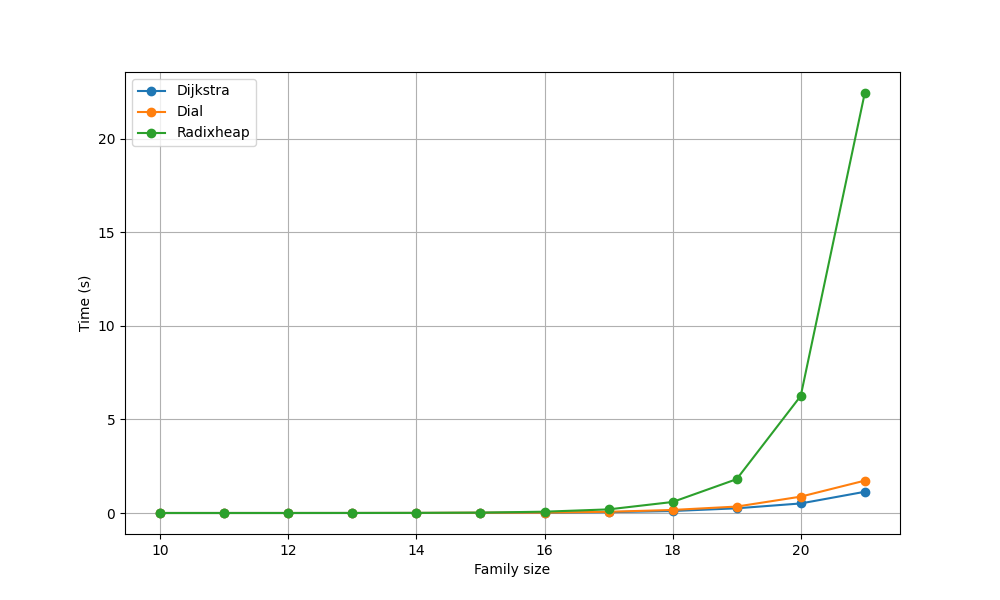
\includegraphics[width=0.9\textwidth]{Random4-n.png}
    \caption{Czas wykonania algorytmów w sekundach dla rodziny \texttt{Random4-n}.}
\end{figure}

\begin{figure}[H]
    \centering
    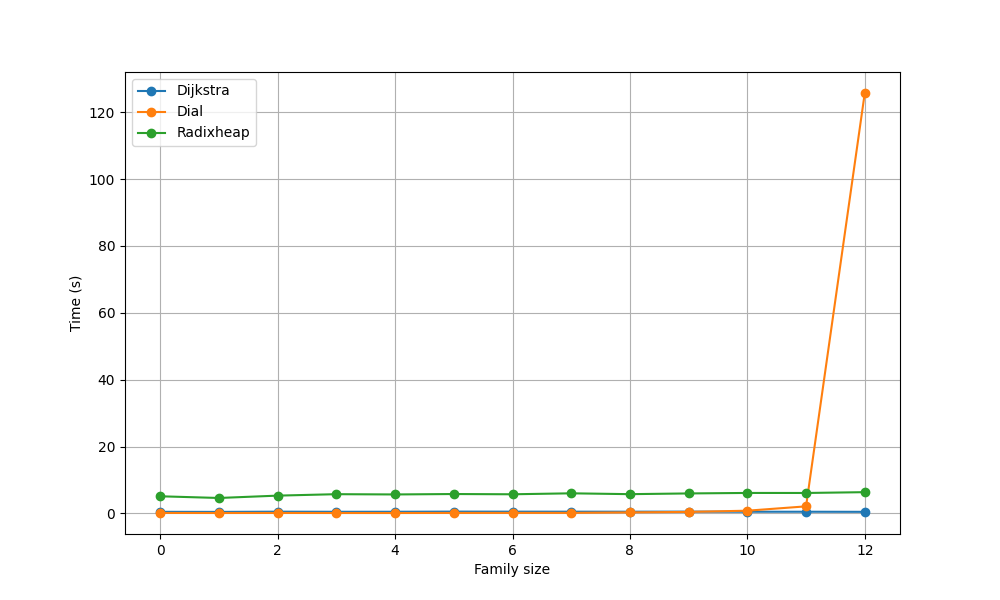
\includegraphics[width=0.9\textwidth]{Random4-C.png}
    \caption{Czas wykonania algorytmów w sekundach dla rodziny \texttt{Random4-C}.}
\end{figure}

\begin{figure}[H]
    \centering
    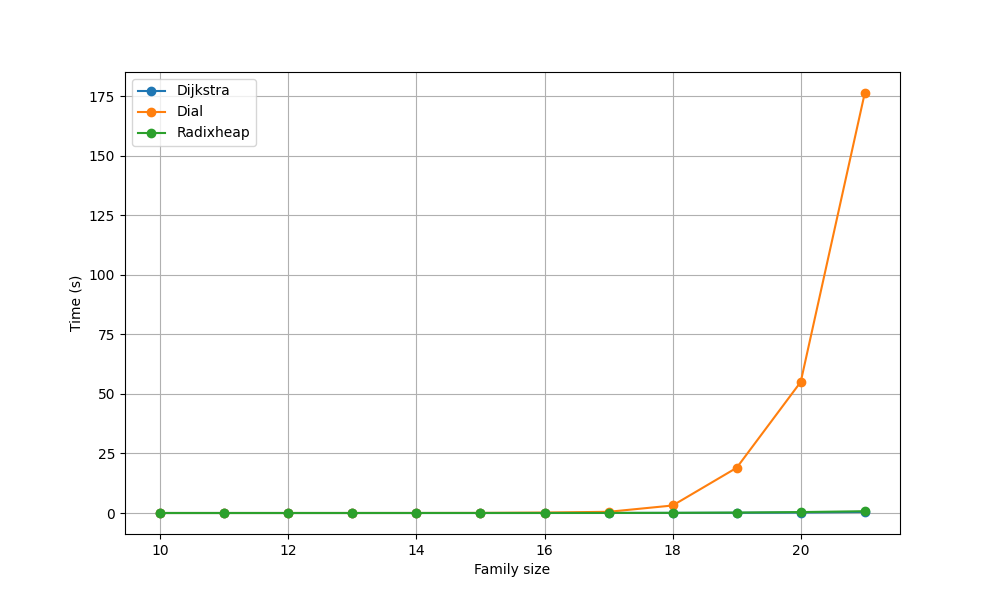
\includegraphics[width=0.9\textwidth]{Long-n.png}
    \caption{Czas wykonania algorytmów w sekundach dla rodziny \texttt{Long-n}.}
\end{figure}

\begin{figure}[H]
    \centering
    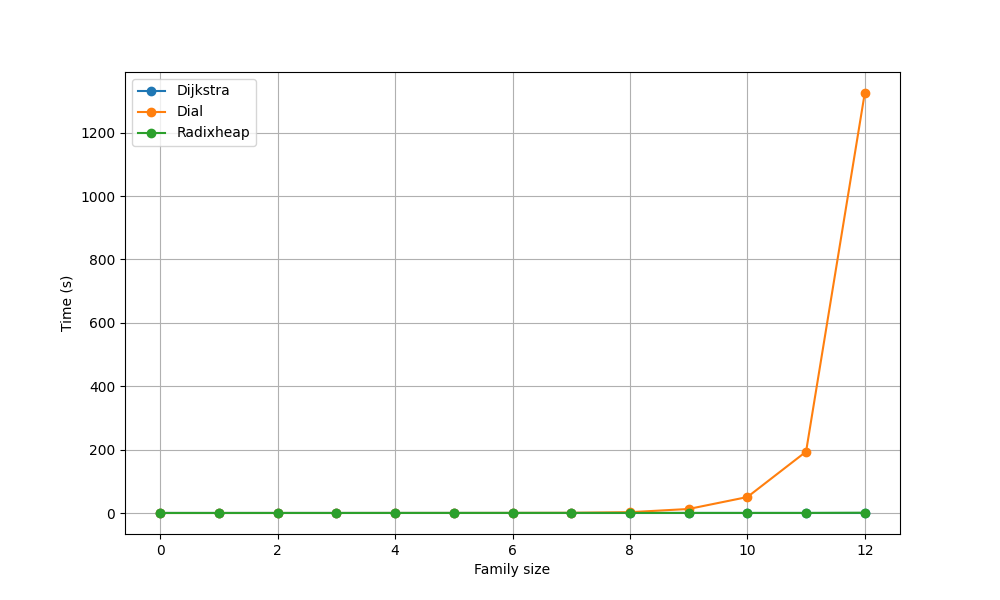
\includegraphics[width=0.9\textwidth]{Long-C.png}
    \caption{Czas wykonania algorytmów w sekundach dla rodziny \texttt{Long-C}.}
\end{figure}

\begin{figure}[H]
    \centering
    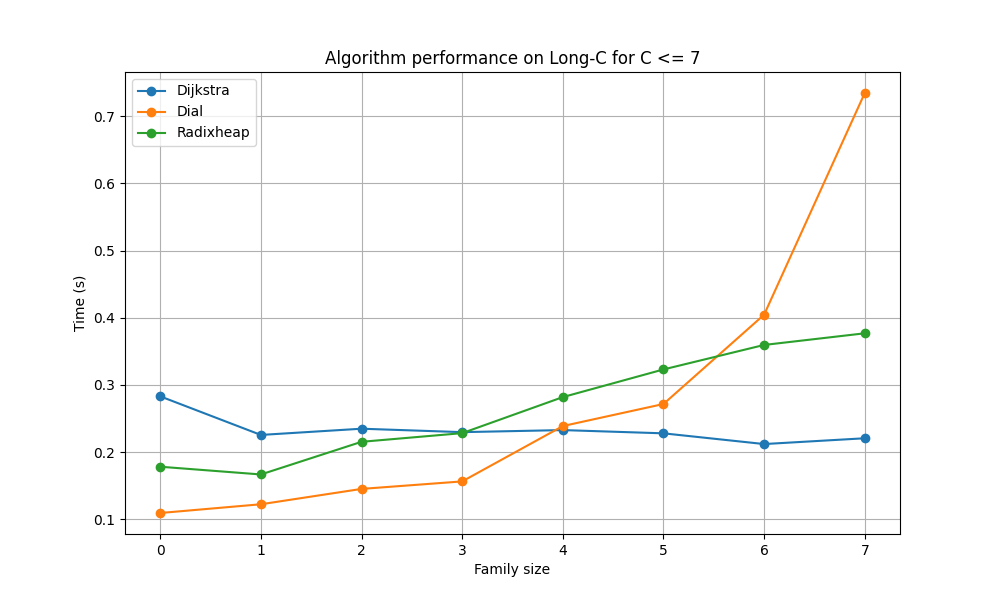
\includegraphics[width=0.9\textwidth]{smaller_Long-C.png}
    \caption{Czas wykonania algorytmów w sekundach dla rodziny \texttt{Long-C} dla $C <= 7$.}
\end{figure}

\begin{figure}[H]
    \centering
    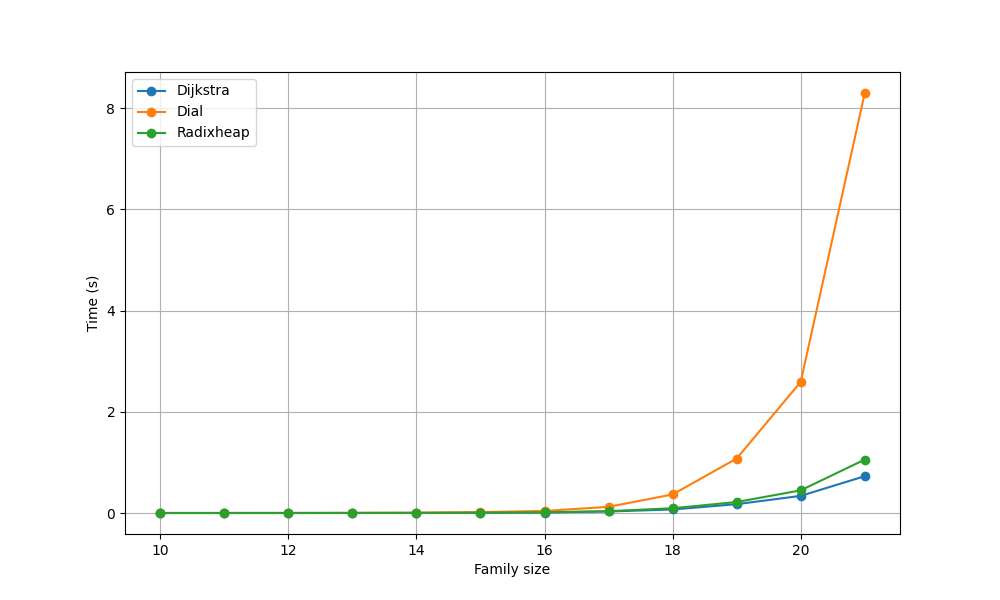
\includegraphics[width=0.9\textwidth]{Square-n.png}
    \caption{Czas wykonania algorytmów w sekundach dla rodziny \texttt{Square-n}.}
\end{figure}

\begin{figure}[H]
    \centering
    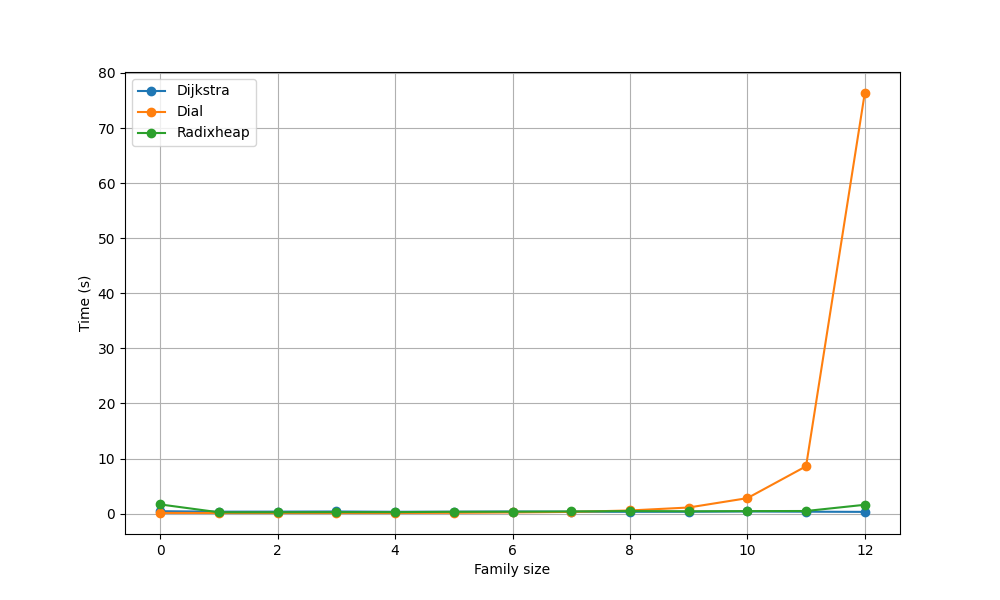
\includegraphics[width=0.9\textwidth]{Square-C.png}
    \caption{Czas wykonania algorytmów w sekundach dla rodziny \texttt{Square-C}.}
\end{figure}

\begin{figure}[H]
    \centering
    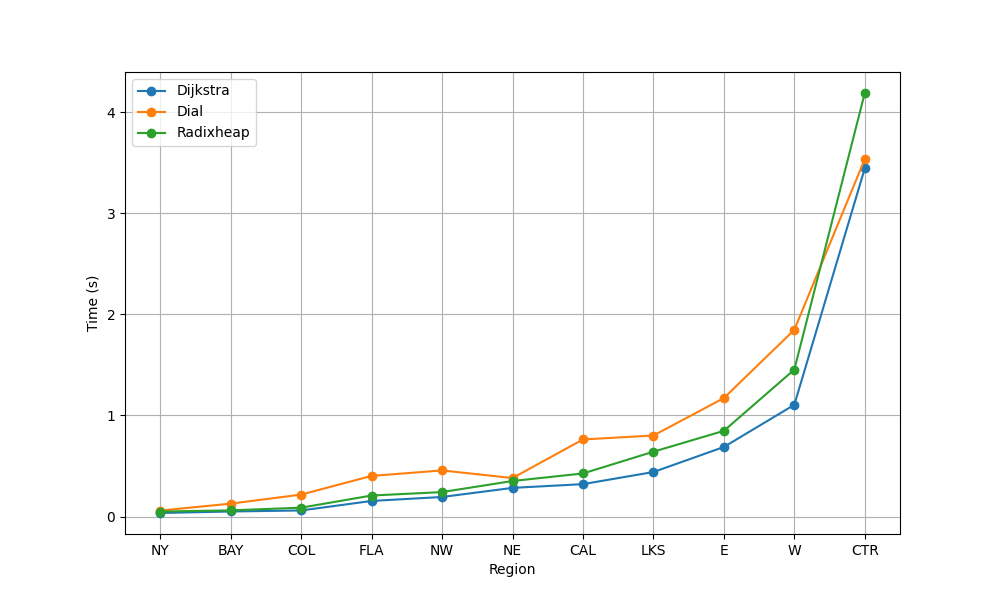
\includegraphics[width=0.9\textwidth]{USA-road-t.png}
    \caption{Czas wykonania algorytmów w sekundach dla rodziny \texttt{USA-road-t}.}
\end{figure}

\subsection{Wyliczone odległości}
Poniżej umieszczam porównanie wyliczonych długości ścieżek dla największych instancji grafów.
Ścieżki zostały wyliczone pomiędzy pierwszym(źródło), a ostatnim wierzchołkiem oraz dla 4 losowych par wierzchołków, innych dla każdego grafu. \\
Ścieżki zostały wyliczone przez wszystkie algorytmy i każdy z nich dał takie same wyniki.

\noindent Losowe wierzchołki dla danych grafów to kolejno:
\begin{itemize}
    \item \texttt{Random4-n-21}: 1064966 $\rightarrow$ 1602932, 903932 $\rightarrow$ 1727836, 287606 $\rightarrow$ 379313, 1365043 $\rightarrow$ 1899558 
    \item \texttt{Random4-C-15}: 146448 $\rightarrow$ 660501, 175713 $\rightarrow$ 788445, 262469 $\rightarrow$ 681208, 604629 $\rightarrow$ 503889
    \item \texttt{Long-n-21}: 701994 $\rightarrow$ 646267, 646686 $\rightarrow$ 652312, 1157387 $\rightarrow$ 201875, 817658 $\rightarrow$ 493825
    \item \texttt{Long-C-15}: 554693 $\rightarrow$ 974335, 571230 $\rightarrow$ 398987, 252889 $\rightarrow$ 5781, 695664 $\rightarrow$ 362215
    \item \texttt{Square-n-21}: 1482318 $\rightarrow$ 1285088, 1268483 $\rightarrow$ 1430604, 401097 $\rightarrow$ 2000552, 887246 $\rightarrow$ 1849742
    \item \texttt{Square-C-15}: 697855 $\rightarrow$ 892182, 381753 $\rightarrow$ 910356, 55396 $\rightarrow$ 525330, 834193 $\rightarrow$ 54688
    \item \texttt{USA-road-t-CTR}: 13366523 $\rightarrow$ 5066525, 7152448 $\rightarrow$ 5676027, 12211682 $\rightarrow$ 9127811, 9092326 $\rightarrow$ 11850392
\end{itemize}

\begin{table}[H]
\centering
\begin{tabular}{|c|c|c|c|c|c|}
\hline
Graf & Pierwszy $\rightarrow$ Ostatni & Losowe 1 & Losowe 2 & Losowe 3 & Losowe 4\\
\hline
\texttt{Random4-n-21} & 9051281 & 10537865 & 9986647 & 8468191 & 7947840\\
\hline
\texttt{Random4-C-15} & 3471241820 & 4506186989 & 4863814130 & 4147135704 & 4397006812\\
\hline
\texttt{Long-n-21} & 31336751771 & 10020735587 & 51646541250 & 33772782005 & 27051220485\\
\hline
\texttt{Long-C-15} & 1308259008765 & 3077736280280 & 4336226283326 & 980237328902 & 1645208124719\\
\hline
\texttt{Square-n-21} & 714640488 & 43699536 & 440808194 & 639663355 & 171077570\\
\hline
\texttt{Square-C-15} & 122219500320 & 75179726868 & 122367430244 & 134415344423 & 119944336220\\
\hline
\texttt{USA-road-t-CTR} & 9709456 & 6377725 & 20532346 & 10927164 & 18794006\\
\hline
\end{tabular}
\caption{Porównanie wyliczonych długości ścieżek dla największych instancji grafów.}
\end{table}

\section{Obserwacje i wnioski}
Patrząc na wykresy, jasno widać, że dla większości rodzin od pewnego etapu algorytm Diala zaczyna mocno odstawać od pozostałych dwóch, pomimo bycia szybkim na początku.
Jego największą wadą jest fakt tworzenia $C + 1$ kubełków, co fatalnie wpływa na jego osiągi dla grafów z dużym $C$.
Jednakże można dostrzec, że ten algorytm również może okazać się przydatny, co widać chociażby dla mniejszych $C$ w rodzinie \texttt{Long-C} - tam algorytm Diala jest najszybszy.

Radix Heap poradził sobie najgorzej na grafie losowym \texttt{n}, gdzie widać dużą różnicę w czasie w stosunku do innych algorytmów.
Jednakże, nie jest ona tak ogromna, jak pomiędzy Dialem, a resztą algorytmów dla dużych $C$.
Jasno widać, że dla grafów z wyższymi wartościami $C$ Radix Heap radzi sobie nieporównywalnie lepiej od Diala, ale wciąż nie lepiej od podstawowego Dijkstry.
Radix Heap nigdzie nie wypadł szczególnie świetnie, ale trzeba pamiętać, że jego implementację można ulepszyć zauważalnie zmniejszająć złożoność.

Podstawowy algorytm Dijkstry dał zadowalające wyniki dla wszystkich testów.
Miał gorsze osiągi jedynie w przypadku grafów z małym $C$. \\

\noindent Można wnioskować, że podstawowy algorytm Dijkstry jest najbezpieczniejszym wyborem, jeśli nie wiemy z jakim grafem przyjdzie nam pracować.
Algorytm Diala i Radix Heap będą odpowiednie dla grafów z małym $C$. Radix Heap poradzi sobie lepiej na grafach z większym zakresem wag, a Dial mniejszym.
Jednakże przy dużych wartościach $C$, koszt organizacji i obsługi kubełków będzie za duży, aby skorzystanie z tych algorytmów miało sens.
W takich wypadkach najlepszy będzie podstawowy algorytm Dijkstry, jako że jego złożoność nie jest zależna od $C$.

\end{document}
